% vim: set foldmethod=marker foldlevel=0:

\documentclass[a4paper]{article}
\usepackage[UKenglish]{babel}

\usepackage{preamble}
\usepackage{array}
\usepackage{tikz}

\renewcommand{\thesubsection}{Q\arabic{section}~(\roman{subsection})}

\fancyhead[L]{MA151 Assignment 1}
\title{MA151 Algebra 1, Assignment 1}

\begin{document}

\maketitle

\setlength{\parindent}{0em}
\setlength{\parskip}{1em}

% {{{ Q1
\question{1}

\subsection{$x \star y = x^2 + y^2,\ S = \mathbb Z$}

This is a binary operation, since it takes two elements of $S$ and always returns another element of $S$. An integer squared plus another integer squared will always be another integer.

\subsection{$x \star y = x + 3,\ S = \mathbb N$}

This is a binary operation, since it takes two elements of $S$ and always returns another element of $S$. A natural number plus 3 is always another natural number.

\subsection{$x \star y = \frac{x + y}{2},\ S = \mathbb Z$}

This is \textit{not} a binary operation, since it takes two elements of $S$ and but doesn't always return another element of $S$. The mean of two integers is not always an integer. Consider $2 \star 3$, for example. $2 \star 3 = \frac{2 + 3}{2} = \frac52 \notin \mathbb Z$.
% }}}

% {{{ Q2
\newquestion{2}

Associativity means that $(a \star b) \star c = a \star (b \star c)$. For the sake of explanation, I shall call the middle term the \textit{pivot term}. So in the case of the example just given, the pivot term was $b$. In the case of $(f \circ (g \circ h)) \circ t = f \circ ((g \circ h) \circ t)$, the pivot term is $(g \circ h)$.

\begin{align*}
	((a \star b) \star (c \star d)) \star e &= (a \star b) \star ((c \star d) \star e) &&\text{pivoting around } (c \star d) \\[1ex]
											&= a \star (b \star ((c \star d) \star e)) &&\text{pivoting around } b \\[1ex]
											&= a \star ((b \star (c \star d)) \star e) &&\text{pivoting around } (c \star d) \\[1ex]
											&= a \star (((b \star c) \star d) \star e) &&\text{pivoting around } c
\end{align*}
% }}}

% {{{ Q3
\question{3}

$$S = \{a, b, c, d\}$$

Call the binary operation $\oplus$. Since $\oplus$ is commutative over $S$, we know that $a \oplus b = b \oplus a$, $d \oplus b = b \oplus d$, etc. So we only need to consider half of the possible combinations. Specifically, we only need to define $a \oplus a$, $a \oplus b$, $a \oplus c$, $a \oplus d$, $b \oplus b$, $b \oplus c$, $b \oplus d$, $c \oplus c$, $c \oplus d$, and $d \oplus d$. Operations like $c \oplus a$ are necessarily given by $a \oplus c$, since $\oplus$ is commutative.

Thus, there are 10 operations to define. Each operation could output any of the 4 elements of $S$, so there are $4^{10} = 1,048,576$ distinct commutative binary operations over $S$.

Most of these operations will not be associative. For example, if $a \oplus b = c$, $b \oplus c = d$, $c \oplus c = a$, and $a \oplus d = b$, then $(a \oplus b) \oplus c = a$ but $a \oplus (b \oplus c) = b$. But the question didn't mention associativity, so this is not something we have to worry about.
% }}}

% {{{ Q4
\newquestion{4}

\subsection{$\left( \left\{ 3^n : n \in \mathbb Z \right\}, \times \right)$}

\begin{enumerate}
	\item A power of 3 multiplied by a power of 3 is always another power of 3, so the group is closed.
	\item Multiplication of integers is associative.
	\item The identity element is $3^0 = 1$.
	\item For some element $3^n$, its inverse is $3^{-n}$, which is also in the set, so inverses exist.
\end{enumerate}

Therefore this is a group.

\subsection{$\left( \left\{ \begin{pmatrix}a & b\\ 0 & c\end{pmatrix} : a, b, c \in \mathbb R \text{ and } ac \ne 0 \right\}, \times \right)$}

\begin{enumerate}
	\item Some matrix $\begin{pmatrix}a & b\\ 0 & c\end{pmatrix}$ multiplied by another matrix $\begin{pmatrix}x & y\\ 0 & z\end{pmatrix}$ equals $\begin{pmatrix}ax & ay + bz\\ 0 & cz\end{pmatrix}$. We note that $ac \ne 0$ and $xz \ne 0$, so $acxz \ne 0$, so this result is in the set and the group is closed under matrix multiplication.
	\item Matrix multiplication is associative.
	\item The identity element is $\begin{pmatrix}1 & 0\\ 0 & 1\end{pmatrix}$, which is definitely in the set, since $1 \times 1 \ne 0$.
	\item The inverse of an element $\begin{pmatrix}a & b\\ 0 & c\end{pmatrix}$ is $\dfrac1{ac} \begin{pmatrix}c & -b\\ 0 & a\end{pmatrix}$. Since $ac \ne 0$, this inverse is well-defined and in the set, so inverses exists in the group.
\end{enumerate}

Therefore this is a group.
% }}}

% {{{ Q5
\newquestion{5}

\subsection{Isosceles triangle}

For the non-equilateral isosceles triangle, the only symmetries are the $0\degree$ rotation (the identity), called $\rho_0$, and the reflection in the vertical line, called $\sigma_0$.

\begin{center}
	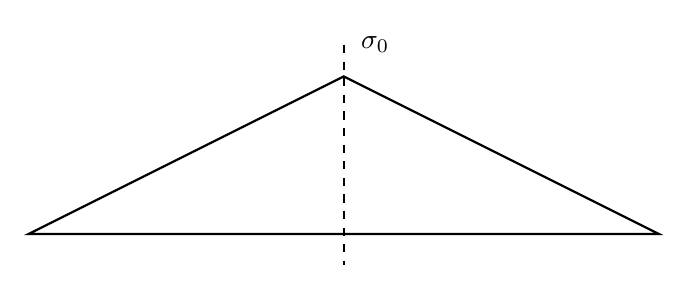
\begin{tikzpicture}[
		scale=2,
		every path/.style={thick}
	]
	\draw (0, 1) -- (2, 0) -- (-2, 0) -- cycle;

	\draw[dashed, semithick] (0, 1.2) -- (0, -0.2);
	\node () at (0.2, 1.2) {$\sigma_0$};
\end{tikzpicture}
\end{center}

And here's the table:
\[
\setlength{\extrarowheight}{3pt}% local setting
\begin{array}{l|*{2}{l}}
    & \rho_0 & \sigma_0 \\
\hline
\rho_0 & \rho_0 & \sigma_0 \\
\sigma_0 & \sigma_0 & \rho_0 \\
\end{array} 
\]

\subsection{Rectangle}

For the non-square rectangle, the only symmetries are the $0\degree$ rotation (the identity), called $\rho_0$, the $180\degree$ rotation, called $\rho_1$, the reflection in the vertical line, called $\sigma_0$, and the reflection in the horizontal line, called $\sigma_1$.

\begin{center}
	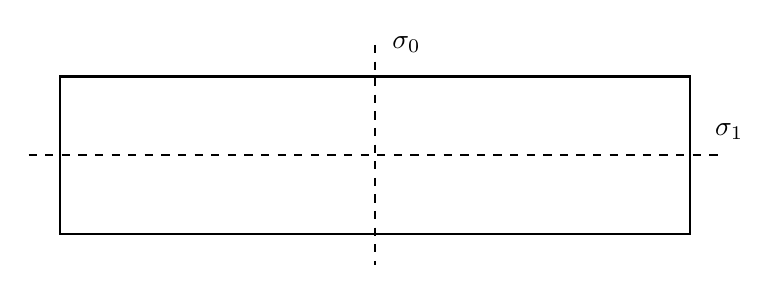
\begin{tikzpicture}[
		scale=2,
		every path/.style={thick}
	]
	\draw (2, 1) -- (2, 0) -- (-2, 0) -- (-2, 1) -- cycle;

	\draw[dashed, semithick] (0, 1.2) -- (0, -0.2);
	\node () at (0.2, 1.2) {$\sigma_0$};

	\draw[dashed, semithick] (-2.2, 0.5) -- (2.2, 0.5);
	\node () at (2.25, 0.65) {$\sigma_1$};
\end{tikzpicture}
\end{center}

And here's the table:
\[
\setlength{\extrarowheight}{3pt}% local setting
\begin{array}{l|*{4}{l}}
	& \rho_0 & \rho_1 & \sigma_0 & \sigma_1 \\
\hline
\rho_0 & \rho_0 & \rho_1 & \sigma_0 & \sigma_1 \\
\rho_1 & \rho_1 & \rho_0 & \sigma_1 & \sigma_0 \\
\sigma_0 & \sigma_0 & \sigma_1 & \rho_0 & \rho_1 \\
\sigma_1 & \sigma_1 & \sigma_0 & \rho_1 & \rho_0 \\
\end{array} 
\]

\section*{Question 6}
\setcounter{section}{6}
\setcounter{subsection}{0}

Let $G$ be a group and let $h \in G$.

\subsection{~}

Let $g_1, g_2 \in G$. If $h g_1 = h g_2$, then we can left-multiply by $h^{-1}$ on both sides to get $h^{-1} h g_1 = h^{-1} h g_2 \implies 1 g_1 = 1 g_2 \implies g_1 g_2$. We know that $h^{-1}$ must exist since $h \in G$ and $G$ is a group.

Conversely, if $g_1 = g_2$, then we can left-multiply by $h$ on both sides and get $h g_1 = h g_2$.

\subsection{~}

Let $S = \{hg : g \in G\}$.

Suppose that $S \ne G$. That means there is some element $a \in G$ which is not in $S$, or there is some element $b \in S$ that was never in $G$.

For the first case, let $a \in G$. Then $h^{-1} a$ is another element of $G$. Thus, $h \left( h^{-1} a \right) = a$, so $a$ must be in $S$. Therefore all elements in $G$ must be in $S$.

For the second case, we know that groups are closed under their binary operation, so $hg$ could never generate a new $b \notin G$. Therefore all elements in $S$ must be in $G$.

Since $G \subset S$ and $S \subset G$, we must conclude that $S = G$.
% }}}

\end{document}
